% !TEX TS-program = pdflatex
% !TEX encoding = UTF-8 Unicode

% This is a simple template for a LaTeX document using the "article" class.
% See "book", "report", "letter" for other types of document.

\documentclass[11pt]{article} % use larger type; default would be 10pt

\usepackage[utf8]{inputenc} % set input encoding (not needed with XeLaTeX)

\usepackage{caption}

%%% Examples of Article customizations
% These packages are optional, depending whether you want the features they provide.
% See the LaTeX Companion or other references for full information.
\usepackage{hyperref}
\usepackage{float}
\usepackage{subfig}

%%% PAGE DIMENSIONS
\usepackage[margin=1.0in]{geometry} % to change the page dimensions
\geometry{a4paper} % or letterpaper (US) or a5paper or....
% \geometry{margin=2in} % for example, change the margins to 2 inches all round
% \geometry{landscape} % set up the page for landscape
%   read geometry.pdf for detailed page layout information

\usepackage{graphicx} % support the \includegraphics command and options

% \usepackage[parfill]{parskip} % Activate to begin paragraphs with an empty line rather than an indent

%%% PACKAGES
\usepackage{booktabs} % for much better looking tables
\usepackage{array} % for better arrays (eg matrices) in maths
\usepackage{paralist} % very flexible & customisable lists (eg. enumerate/itemize, etc.)
\usepackage{verbatim} % adds environment for commenting out blocks of text & for better verbatim
\usepackage{subfig} % make it possible to include more than one captioned figure/table in a single float
% These packages are all incorporated in the memoir class to one degree or another...
\setlength{\parskip}{0.5em}

%%% HEADERS & FOOTERS
\usepackage{fancyhdr} % This should be set AFTER setting up the page geometry
\pagestyle{fancy} % options: empty , plain , fancy
\renewcommand{\headrulewidth}{0pt} % customise the layout...
\lhead{}\chead{}\rhead{}
\lfoot{}\cfoot{\thepage}\rfoot{}

%%% SECTION TITLE APPEARANCE
\usepackage{sectsty}
\allsectionsfont{\sffamily\mdseries\upshape} % (See the fntguide.pdf for font help)
% (This matches ConTeXt defaults)
%%% ToC (table of contents) APPEARANCE
\usepackage[nottoc,notlof,notlot]{tocbibind} % Put the bibliography in the ToC
\usepackage[titles,subfigure]{tocloft} % Alter the style of the Table of Contents
\renewcommand{\cftsecfont}{\rmfamily\mdseries\upshape}
\renewcommand{\cftsecpagefont}{\rmfamily\mdseries\upshape} % No bold!

%%% END Article customizations

%%% The "real" document content comes below...

\title{Software Engineering Project Weekly Report\\ \textbf{3D-KORN} \\ University of Bourgogne}
\author{Luca Canalini \and Ezequiel De La Rosa \and Benjamin Lalande Chatin \and Roberto Paolella \and Umamaheswaran Raman Kumar \and Savinien Bonheur \and Albert Clerigues Garcia \and Daniel Gonzalez Adell \and Nayee Muddin Khan Dousai \and Pamir Ghimire \and Di Meng
}

\date{Nov 14, 2016} % Activate to display a given date or no date (if empty),
%         % otherwise the current date is printed 

\begin{document}
\maketitle
\newpage
\section{Tasks completed}
	Each working group has created its own class with the main functions developed since now. 
	The classes are as follow:
	
\begin{itemize}

	\item \textbf{Scan Registration Class} $(Albert, Ezequiel)$
	\begin{itemize}
		\item \textit{Uniformly downsampling function} (\textin{using} $VoxelGrid Filter)$ takes as input the original Point Cloud and downsamples it to about $10 \% $ of the points.
		\item \textit{Rough Alignment Function} using sample alignment consesus $(SAC)$ 
		\item \textit{ICP Alignment Function}	
	\end{itemize}
	
	\begin{center}
		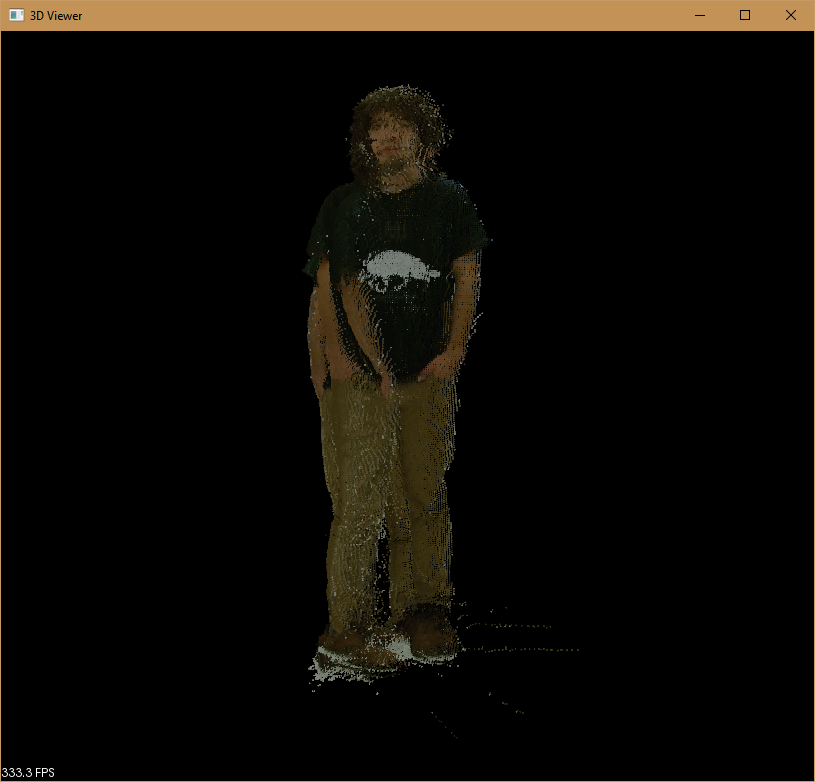
\includegraphics[scale = 0.25]{ScanR1.png} 
		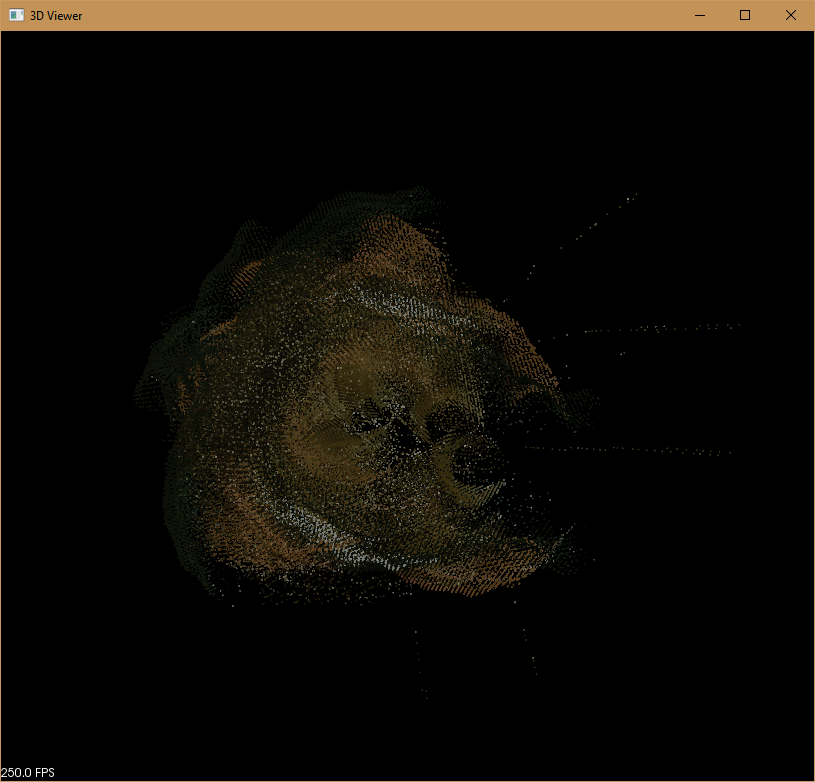
\includegraphics[scale = 0.25]{ScanR2.png}
		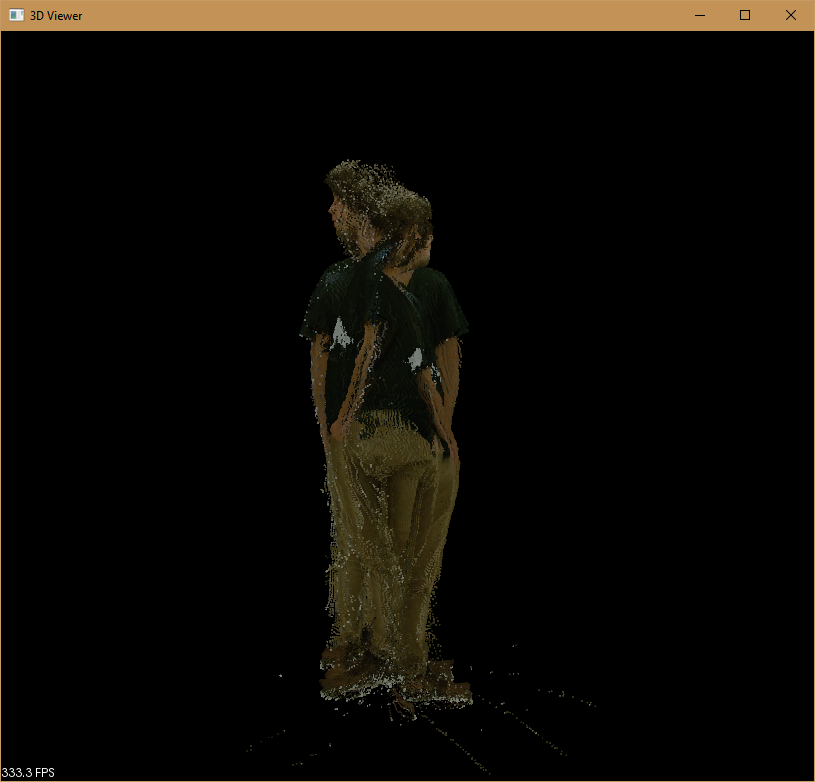
\includegraphics[scale = 0.25]{ScanR3.png} 	
		
	\end{center}
	
	
	\item \textbf{Point Cloud Operations Class} $(Savinien,Luca,Roberto,MengDi)$
		\begin{itemize}
			\item \textit{Conversion Function} of Point Cloud object from type $<XYZRGB>$ to type $<XYZ>$
			\item \textit{Passthrough Filter function}
			\item \textit{Normal Estimation function}
			\item \textit{Poisson Meshes function} takes in input the original Point Cloud and gives in output a mesh using all the fucntion that we presented above.
		
		
		\end{itemize}
		
			\begin{center}
				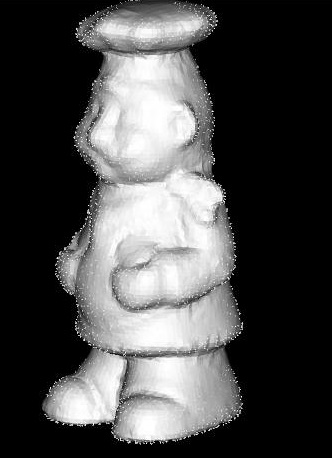
\includegraphics[scale = 0.5]{PoinOp3.png} 
				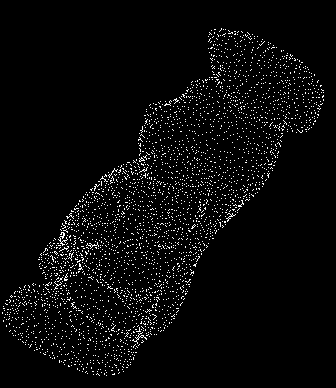
\includegraphics[scale = 0.5]{PoinOp1.png}	
				
			\end{center}	
	
	\item \textbf{GUI Class} $(Nayeem,Benjamin,Umamaheswaran)$
		\begin{itemize}
			\item Load pointcloud in the GUI using QVTK Widget.
			\item Login, Menu and Status Bar.
		\end{itemize}
\begin{center}
        
		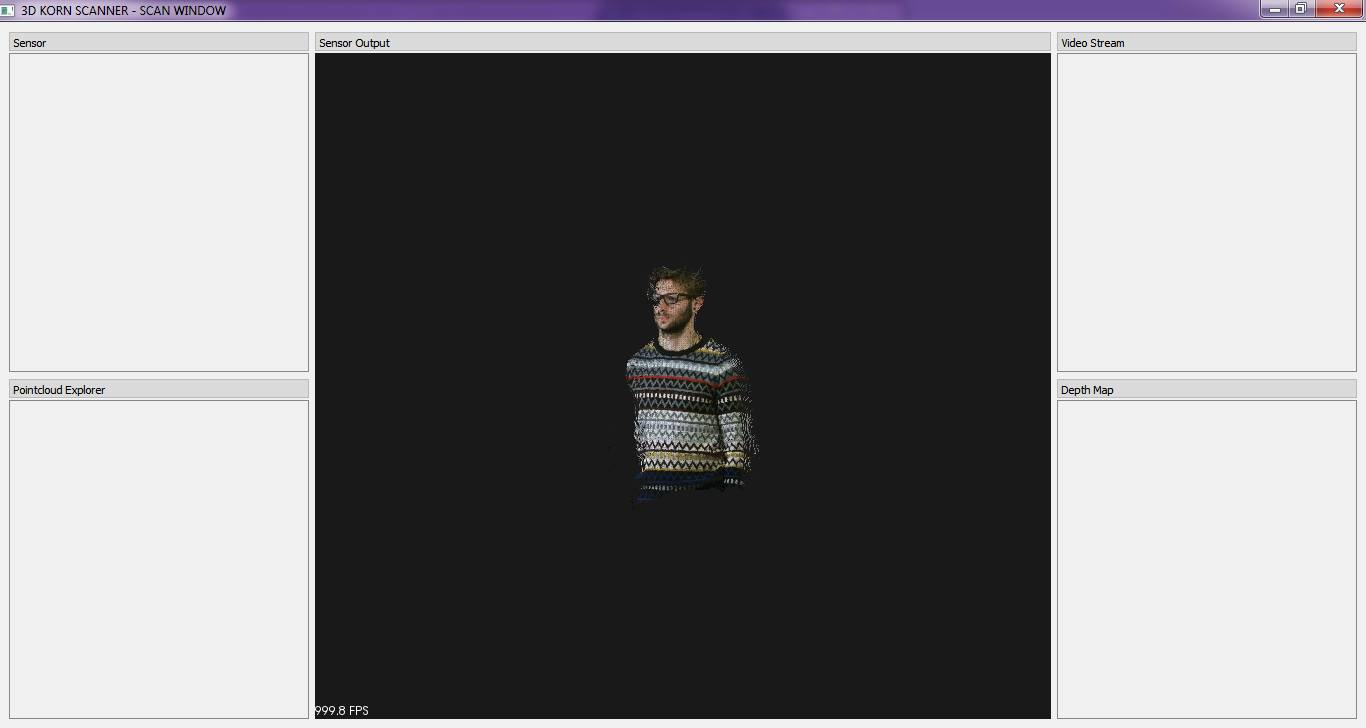
\includegraphics[scale = 0.3]{GUI1.png} 
	
	
\end{center}
		
	
	
	
	\item \textbf{Kinect Contreller Class} $(Pamir,Dani)$\\
	This group has already implemented the following functions and they are currently working on the class' implementation
	\begin{itemize}
		\item \textit{Start/Stop Grabber function} 
		\item \textit{RGB Video Stream/Image Get function}
		\item \textit{Point Cloud Get function}
	\end{itemize}
	
	\begin{center}
		
		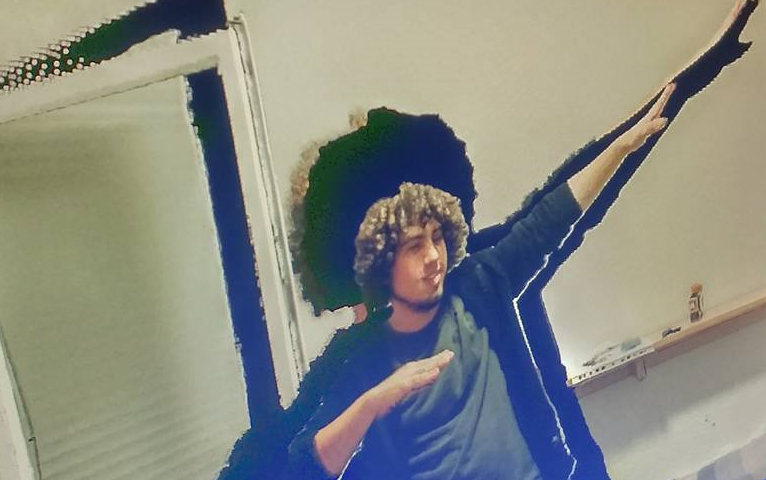
\includegraphics[scale = 0.3]{Kinect.png} 
		
		
	\end{center}
	
	
\end{itemize}

\section{Main Goal For Coming Week}

\begin{itemize}

\item Start integration of all the code together for first testing

\item Create the presentation that will be held for the first demo


\item Each group will start to implement new features inside its own class:
\begin{itemize}
	
	\item \textbf{Scan Registration Class} 
	\begin{enumerate}
		\item Improve the registration process with different approach.
	\end{enumerate}
	
	
	\item \textbf{Point Cloud Operations Class}
\begin{enumerate}
	\item Create color meshes.
\end{enumerate}

	\item \textbf{GUI class}
	\begin{enumerate}
		\item Work on Live Video Streaming.
		\item Divide the main GUI class into subclasses.
	\end{enumerate}

	\item \textbf{Kinect Controller Class}
	\begin{enumerate}
		\item Finish the implementation of the class.
		\item Current video stream from point cloud $<XYZRGB>$.
		\item Get pure $RGB$ stream.
	\end{enumerate}
	
\end{itemize}




\end{itemize}

\section{Important links}
\begin{itemize}
\item Task allocation and progress  (\url{https://goo.gl/WDHEjf)}
\item Github repository (\url{https://github.com/umaatgithub/3D-KORN})
\item Group's work Integration Branch  (\url{https://github.com/umaatgithub/3D-KORN/tree/integration-branch/Source-Code}) 
\end{itemize}



\end{document}


